\documentclass{amsart}

\usepackage[T1]{fontenc}
\usepackage[utf8]{inputenc}
\usepackage[UKenglish]{babel}
\usepackage{amsmath}
\usepackage{amsthm}
\usepackage{amssymb}
\usepackage{float}
\usepackage{graphicx}
\usepackage{algorithm}
\usepackage{algorithmic}
\usepackage{todonotes}
\usepackage{enumitem}
\usepackage[misc]{ifsym}
\usepackage[foot]{amsaddr}
\usepackage[hidelinks]{hyperref}
\usepackage{csquotes}
\usepackage[style=authoryear,ibidtracker=false,uniquename=false,giveninits=true,terseinits=true,maxbibnames=5,backend=biber]{biblatex}
\renewbibmacro{in:}{}
\addbibresource{rnni_convexity.bib}

\newcommand{\np}{\mathcal{NP}}
\newcommand{\parent}{\mathrm{parent}}
\newcommand{\mrca}{\mathrm{mrca}}
\newcommand{\rank}{\mathrm{rank}}
\newcommand{\nni}{\mathrm{NNI}}
\newcommand{\rnni}{\mathrm{RNNI}}
\newcommand{\rnniu}{\mathrm{RNNIu}}
\newcommand{\tbr}{\mathrm{TBR}}
\newcommand{\spr}{\mathrm{SPR}}
\newcommand{\csort}{\textsc{Caterpillar Sort}}
\newcommand{\findpath}{\textsc{FindPath}}
\newcommand{\mdtree}{\textsc{MDTree}}

\newtheorem{definition}{Definition}
\newtheorem{theorem}[definition]{Theorem}
\newtheorem{conjecture}[definition]{Conjecture}
\newtheorem{lemma}[definition]{Lemma}
\newtheorem{corollary}[definition]{Corollary}
\newtheorem{proposition}[definition]{Proposition}

\graphicspath{{figures/}}

\sloppy


\title[Ranked Nearest Neighbour Intarchange]{Geometry of Ranked Nearest Neighbour Interchange Space of Phylogenetic Trees}
\date{\today}
\author{Lena Collienne\textsuperscript{1}}
\email{lena.collienne@postgrad.otago.ac.nz}
\address{\textsuperscript{1}Department of Computer Science, University of Otago, New Zealand}
\author{Mareike Fischer\textsuperscript{2}}
\email{email@mareikefischer.de}
\address{\textsuperscript{2}Institute for Mathematics and Inofrmatics, University of Greifswald, Germany}
\author{David Bryant\textsuperscript{3}}
\email{david.bryant@otago.ac.nz}
\address{\textsuperscript{3}Department of Mathematics and Statistics, University of Otago, New Zealand}
\author{Alex Gavryushkin\textsuperscript{1, \Letter}}
\email{\textsuperscript{\Letter}alex@biods.org}


\begin{document}


\begin{abstract}
In this paper we study the graph of ranked phylogenetic trees where the adjacency relation is given by a local rearrangement of the tree structure.
Our work is motivated by tree inference algorithms, such as maximum likelihood and Markov Chain Monte Carlo methods, where the geometry of the search space plays a central role for efficiency and practicality of the optimisation.
We hence focus on understanding the geometry of the space (graph) of ranked trees, the so-called ranked nearest neighbour interchange ($\rnni$) graph.
Specifically, we introduce some algorithms for computing paths in the $\rnni$ graph and use them to establish properties such as diameter and radius of this graph.

We also study the problem of computing distances between trees in this graph.
Since the $\rnni$ graph is a generalisation of the classical nearest neighbour interchange ($\nni$) graph to ranked phylogenetic trees, we specifically focus on the properties that have already been established for $\nni$.
Surprisingly, our results suggest that the complexity of computing distances in the two graphs is likely to be different.
%TODO
% Alex: The proof for $\np$ hardness of $\nni$ uses trees that have two caterpillar trees as subtrees (See Fig5).
% I'm not sure whether it's known that computing distances just between caterpillar trees is not polynomial in $\nni$.
% Do I need to be more specific about this here?
% And shall I use the term 'caterpillar trees' here?
We prove that within a particular subset of trees distances can be computed in polynomial time in $\rnni$ while this is not known to be true in $\nni$.
\end{abstract}


\maketitle

The nearest neighbour interchange ($\nni$) graph, defined on the set of phylogenetic trees with adjacency relation given by the interchange operation of two sister clades, has been known in mathematical biology literature for nearly 50 years \autocite{Robinson1971-ql,Moore1973-kk}.
Considered with the metric given by the length of a shortest path (graph-distance), this graph becomes a metric space.
Its geometry has been extensively studied \autocite{Dasgupta2000-xa, Li1996-zw, Gordon2013-fw, De_Jong2016-al}.
An important property of the $\nni$ graph is that computing distance is NP-hard \autocite{Dasgupta2000-xa}.
As a result no algorithm exists to compute the distance in practical time.
A consequence is that tree search and sampling algorithms pose a significant challenge even for moderately sized trees
\autocite{Whidden2016-kl}.

More recent advances in computational phylogenetics introduce various classes of molecular clock models \autocite{Yoder2000-ks,Drummond2006-nl,Drummond2010-yf} and made computational inference of phylogenetic time-trees possible \autocite{Ronquist2003-eq, Bouckaert2018-yr, Hadfield2018-xp}.
However, mathematical challenges that come with this seemingly inessential change in parametrisation (genomic distance VS time distance) of trees have only recently been brought to attention \autocite{Gavryushkin2016-uu}.
These differences motivated \textcite{Gavryushkin2018-ol} to propose an extension of the $\nni$ graph to the class of discrete time-trees.
The simplest such extension introduces the $\rnni$ graph on the set of ranked phylogenetic trees.
Considered with the graph-distance $\rnni$ becomes a metric space and inherits the geometric and algorithmic challenges that the $\nni$ space has been traditionally facing.
Surprisingly, most of them cannot be settled by directly translating results or applying techniques developed for $\nni$ \autocite{Gavryushkin2018-ol}.

In this paper, we consider the $\rnni$ space on ranked phylogenetic trees with all taxa being of equal rank.
An example of such a tree is depicted in Figure~\ref{fig:ranked_tree}.
In the terminology of \autocite{Gavryushkin2018-ol}, the space considered in this paper is the space of ranked ultrametric phylogenetic trees $\rnniu$.
We postpone accurate definitions until later in this section.

\begin{figure}[H]
\centering
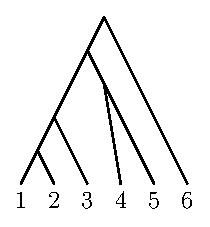
\includegraphics[width=0.25\textwidth]{ranked_tree}
\vspace{12pt}
\caption{A ranked tree with $6$ taxa.}
\label{fig:ranked_tree}
\end{figure}

In line with the research programme proposed in \autocite{Gavryushkin2018-ol}, we investigate the geometry and algorithmic complexity of the $\rnni$ space.
Specifically, in this paper we establish the exact radius and diameter of the space (Section~\ref{section:diameter}).
We also show that the subset of caterpillar trees is convex in $\rnni$ (Section~\ref{section:caterpillar_convex}), thus settling one of the open problems proposed in \autocite{Gavryushkin2018-ol}.
For establishing these geometric properties we are using algorithms that will be introduced in Section~\ref{section:algorithms}.
We will in particular provide an approximate algorithm that computes exact distances for small trees.
The question of whether there exists a polynomial algorithm for computing the $\rnni$ distance remains an open problem.

In the rest of this chapter we formally introduce the terminology used in this paper.

A \emph{ranked phylogenetic tree} is a pair consisting of a rooted binary phylogenetic tree $T$ on the set $X = \{1, \ldots, n\}$ of \emph{taxa} for $n \in \mathbb N$, and a (total) rank function that maps all leaves of $T$ to $0$, all internal nodes of $T$ onto elements of the set $\{1, \ldots, n-1\}$, and respects the partial order on the nodes given by the tree.
The latter means that if $u$ and $v$ are two internal nodes of $T$ such that there exists a path from a taxon $x \in X$ to the root which first passes through $u$ and then through $v$ then $\rank(u) < \rank(v)$.
Ranked trees $(T_1, \rank_1)$ and $(T_2, \rank_2)$ are different if trees $T_1$ and $T_2$ are different or $T_1 = T_2$ and $\rank_1 \neq \rank_2$.
Since all trees in this paper are ranked trees, we will abuse the notation and drop the rank function from the notation.
We will also simply say trees to mean ranked phylogenetic trees.
For a tree $T$, we will use $\rank_T$ to refer to its ranking.
A ranked tree $T$ without its leaf labels will be called \emph{tree topology}.

Our definition of a ranked tree implies a natural notion of edge length -- we call $|\rank_T(v) - \rank_T(u)|$ the length of an edge $(u, v)$.

Now we are ready to introduce the tree space which is the subject of study in this paper, the $\rnni$ graph.

The vertex set of the $\rnni$ graph is the set of all ranked trees on $n$ taxa.
We introduce two types of operation ($\rnni$ \emph{moves}) on trees (see Figure~\ref{fig:RNNI}) and say that two trees are adjacent in the $\rnni$ graph if they are connected by an operation of either type.
The first type of operation is called a \emph{rank move} and defined by swapping the ranks of two internal nodes that are not adjacent in the tree.
Formally, if $u$ and $v$ are nodes of a tree $T$ such that $|\rank_T(u) - \rank_T(v)| = 1$ and $(u, v)$ is not an edge in $T$ then the tree $R$ obtained from $T$ by only changing $\rank_R(u) = \rank_T(v)$ and $\rank_R(v) = \rank_T(u)$ is said to be obtained by a rank move.
The second type of operation is called an $\nni$ \emph{move} and defined in the usual way, that is, two trees $T$ and $R$ are said to be connected by an $\nni$ move if there exist internal edges $e$ in $T$ and $f$ in $R$ both of length one such that the trees obtained by shrinking $e$ and $f$ to internal nodes coincide.

We use the notation $d(T, R)$ throughout the paper to denote the graph distance between trees in $\rnni$, that is, $d(T, R)$ is the length of a shortest $\rnni$ path between tree $T$ and $R$.

\begin{figure}[H]
\centering
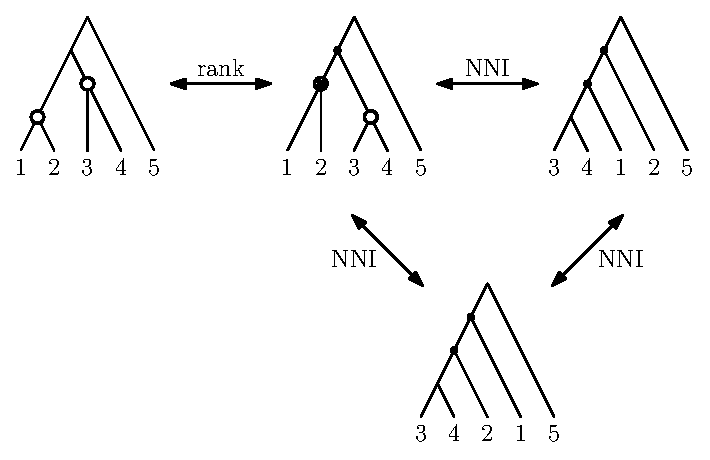
\includegraphics[width=0.8\textwidth]{RNNI}
\vspace{12pt}
\caption{Two types of operation that define edges of the $\rnni$ graph.
The rank move swaps the rank of the two highlighted nodes and the $\nni$ moves are performed on the blue edges.}
\label{fig:RNNI}
\end{figure}

The rest of this paper is structured as follows.
Within the next section we introduce three algorithms for exploring the $\rnni$ graph.
We use these algorithms in Section~\ref{section:geometry} for proving some geometrical properties of this graph, such as diameter and radius.
Specifically, we will prove in Section~\ref{section:caterpillar_convex} that for a subset of $\rnni$ trees, distances can be computed in polynomial time.
This already suggests that there is a difference in complexity of computing distances between the $\rnni$ graph and the classical $\nni$ graph.
\todo{Alex: Is it OK to use 'shortest $\rnni$ paths' here?}
We will discuss this further in Section~\ref{section:cluster_theorem} where we disprove a conjecture raised in \autocite{Gavryushkin2018-ol} and provide an alternative version, which makes a claim about the similarity of trees on shortest $\rnni$ paths.


\section{Algorithms}
\label{section:algorithms}

In this section we introduce three algorithms, $\findpath$ (Section~\ref{section:alg_findpath}), $\csort$ (Section~\ref{section:alg_csort}), and $\mdtree$ (Section~\ref{section:alg_mdtree}).
$\findpath$ computes a $\rnni$ path between trees.
$\csort$ computes a shortest $\rnni$ path between caterpillar trees (also known as ladder trees, see later in this section for accurate definitions).
$\mdtree$ maximises the dissimilarity to find a remote tree given an arbitrary $\rnni$ tree.
While these algorithms are interesting on their own (e.g.\ in simulation studies), they will also form an important ingredient to study the geometry of the $\rnni$ space later in this paper.

The algorithm $\findpath$ can be used to approximate the $\rnni$ distance.
We will study the accuracy of this approximation by computing the exact $\rnni$ distance for small trees.
Specifically, we will use the algorithm for computing the complete $\rnni$ graph that is given in \autocite[their Section 3.3]{Gavryushkin2018-ol}.
After pre-computing the graph, we use the standard algorithms~\autocite{Floyd1962-ew,Dijkstra1959-ph} for computing shortest paths.
However, the large number of vertices in $\rnni$ is an obstacle when it comes to computing distances for larger trees.
Since there are $\frac{n!(n-1)!}{2^{n-1}}$ vertices in the $\rnni$ graph \autocite{Gavryushkin2018-ol}, we compute the $\rnni$ graph on up to six taxa for our analyses.
This computational result will also be used later in the paper to support Conjecture~\ref{conjecture:cluster_theorem}, a modification of Conjecture~9 in \autocite{Gavryushkin2018-ol}, which we prove to be false in this paper.
Our implementations can be found on GitHub in \autocite{Collienne2019}.


\subsection{$\findpath$}
\label{section:alg_findpath}

In this section we present $\findpath$, an efficient algorithm for computing paths, and therefore approximating distances, between trees in $\rnni$.

Before introducing the algorithm we need the following definitions.
Each node $v$ of a tree defines a \emph{cluster} $C$, which is the set of taxa descending from $v$.
We then say that $v$ \emph{induces} $C$.
\emph{Trivial clusters} are clusters induced by leaves (contain just one element each) and the root of the tree (contains all taxa).
As all trees on $n$ taxa share all trivial clusters, we will use the notion cluster to mean non-trivial clusters.
Note that the list of all non-trivial clusters of a tree, sorted according to the rank of the corresponding node, defines the tree unambiguously.
We will refer to this list of $n-2$ clusters for a given tree on $n$ taxa as a \emph{cluster representation} of the tree.

Let $T$ and $R$ be arbitrary trees and $[C_1, \ldots, C_{n-2}]$ be the cluster representation of $R$ (the ``destination'' tree).
Then $C_i$ is induced by the node of rank $i$ for $i = 1, \ldots, n-2$.
$\findpath$ computes a path by iteratively extending a sequence $p$ of trees starting from $T$.
The algorithm terminates when $p$ is an $\rnni$ path from $T$ to $R$.

\todo{Alex: go through the following two paragraphs and proof of L1}
In step $k$ of $\findpath$ we consider the cluster $C_k$ for $k = 1, \ldots, n-2$.
$p$ is extended in step $k$ by considering the last tree $T'$ on $p$ and finding the node in $T'$ that induces the smallest cluster containing all elements of $C_k$.
This node is denoted by $\mrca_{T'}(C_k)$ (short for \emph{most recent common ancestor}).
By performing an $\rnni$ move that decreases the rank of $\mrca_{T'}(C_k)$, we receive a tree that is then appended to $p$.
Now we extend $p$ by repeatedly performing $\rnni$ moves on the last tree of $p$ that move the most recent common ancestor of $C_k$ down.
In the end of step $k$, $C_k$ is induced by the internal node of rank $k$ in the last tree of $p$.

By following this procedure, the last of $p$ after step $n-2$ will be $R$, as it contains all clusters of $R$.
It is important but easy to see that the output path of $\findpath$ is unique for a given pair of trees, which means that it is a deterministic algorithm.
This is due to the fact that there exists exactly one $\rnni$ move that decreases the rank of the most recent common ancestor of a subset $C_k$ of the taxon set of a tree as long as $C_k$ is not induced by an internal node of that tree.

\begin{algorithm}[H]
\caption{$\findpath$($T,R$)}
\label{alg:find_path}
\begin{algorithmic}[1]
\STATE $T' := T$
\STATE $p := [T']$
\FOR {$k = 1, \dots, n-2$}
\STATE Let $C_k$ be the cluster induced by the node with rank $k$ in $R$ \label{alg:find_path:line:cluster}
\WHILE {$\rank_{T'}(\mrca_{T'}(C_k))>k$}
\STATE Update $T'$: Decrease $\rank_{T'}(\mrca_{T'}(C_k))$ by an $\rnni$ move \label{alg:findpath:line:move_set_down}
\STATE $p = p+T'$
\ENDWHILE
\ENDFOR
\RETURN $p$
\end{algorithmic}
\end{algorithm}

The following lemma shows that $\findpath$ is correct, that is, the algorithm returns a path between the two input trees.
To prove this we have to establish that there always exists a unique $\rnni$ move required in Line~\ref{alg:findpath:line:move_set_down} of the algorithm.

\begin{lemma}
Let $T = [C_1, \ldots, C_{k-1}, B_{k}, \ldots, B_{n-2}]$ and $R = [C_1, \ldots, C_{k-1}, C_k, \ldots, C_{n-2}]$ be two trees where $C_k \neq B_k, \ldots, B_{n-2}$.
Then there exists exactly one $\rnni$ move on $T$ that results in a tree $T'$ such that $\mrca_{T'}(C_k) < \mrca_{T}(C_k)$.
\label{lemma:mrca_move}
\end{lemma}

\begin{proof}
Let $T$ and $R$ be trees as defined in the lemma.
Notice that the only $\rnni$ move on $T$ that could decrease the rank of $\mrca_T(C_k)$ are $\nni$ moves on the edge between $\mrca_T(C_k)$ and its child (if this edge has length one), or a rank move between $\mrca_T(C_k)$ and the node with rank one less.
Therefore, we will now distinguish these two cases:
Either there is an edge $(v,w)$ between nodes $v = \mrca_T(C_k)$ and $w$ with rank $rank_T(w) = rank_T(v) - 1$, or there is no such edge.

In the latter case the only $\rnni$ move that could decrease the rank of $v$ is a rank move swapping the ranks of $v$ and $w$.

Let us now assume that there is an edge $(v,w)$ in $T$.
Let $T_v$ be the subtree that is rooted in the child of $v$ that is not $w$ and let $T_{w_1}$ and $T_{w_2}$ be the subtrees rooted in the children of $w$.
We are now going to explain why only one of these two $\nni$ moves changes the rank of $\mrca_T(C_k)$.
It is important to notice that $C_k$ either is the disjoint union of two of the clusters $C_1, \ldots, C_{k-1}$ or the union of one of those clusters with a single taxon that is not included in any of those clusters.
In general we can say that $C_k = S_1 \dot\cup S_2$ is the union of two subsets of taxon set of $T$ such each of these subsets is contained in one of the subtrees $T_v, T_{w_1}$, or $T_{w_2}$.
In fact, $S_1$ and $S_2$ are contained in two different of these subtrees.
Now it is easy to see that just one of the $\nni$ moves on $(v,w)$ (illustrated in Figure~\ref{fig:mrca_move}) decreases the rank of $\mrca_T(C_k)$.

\begin{figure}[H]
\centering
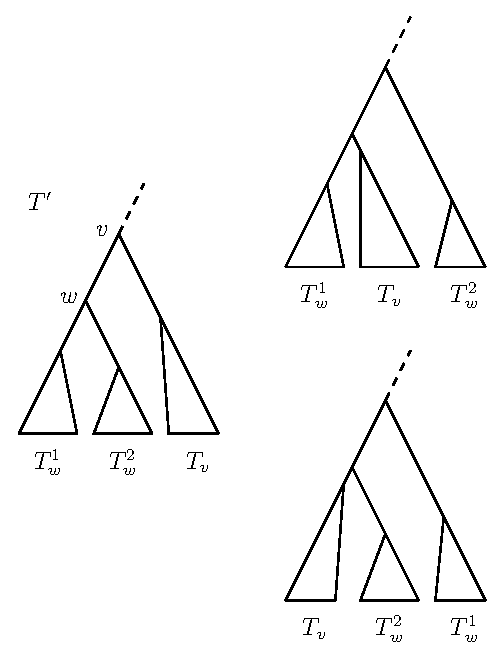
\includegraphics[width=0.5\textwidth]{mrca_move}
\vspace{12pt}
\caption{Two $\nni$ moves that are possible on the edge $(v,w)$ of the tree $T'$ with subtrees $T_v, T_{w_1}, T_{w_2}$ as described in the proof of Lemma~\ref{lemma:mrca_move}.}
\label{fig:mrca_move}
\end{figure}
\end{proof}

Note that the uniqueness of the $\rnni$ move in Line~\ref{alg:findpath:line:move_set_down} of the algorithm $\findpath$ also implies that the algorithm is deterministic.
The running time of the algorithm is quadratic in the number of taxa.

Because the algorithm returns a path between pairs of trees in $\rnni$, the length of the path approximates the $\rnni$ distance from above.
A natural question then is how accurate this approximation is.
We have computationally shown that the algorithm $\findpath$ finds the correct distance for trees up to six taxa.
Specifically, we have implemented $\findpath$ \autocite{Collienne2019} and compared the results with the true $\rnni$ distance as explained earlier in this section.


\subsection{$\csort$}
\label{section:alg_csort}

In this section we introduce an algorithm to compute paths between \emph{caterpillar trees}, which are trees where each internal node is adjacent to at least one leaf.
As a result caterpillar trees have only one \emph{cherry}, which is a pair of taxa that share their parent.
A path between two caterpillar trees that only consists of caterpillar trees is called a \emph{caterpillar path}.
We can identify a caterpillar tree $T = [\{x_1, x_2\}, \{x_1, x_2, x_3\}, \ldots, \{x_1, \ldots, x_n\}]$ with the list of its taxa $[x_1, x_2, \ldots, x_n]$, assuming that $x_1 < x_2$ as natural numbers (recall that the set of taxa is $\{1, \ldots, n\}$).

The algorithm $\csort$ (Algorithm~\ref{alg:csort}) is a natural modification of the classical \emph{Bubble Sort} algorithm \autocite{Knuth1997-pi}.
A path $p$ from $T$ to $R= [x_1, x_2, \ldots, x_n]$ is computed iteratively such that after $k$ steps the last $k$ taxa of $T$ and $R$ coincide.
Specifically, in step $k$ ($k = 0, \ldots, n-3$) taxon $x_{n-k}$ is moved up to the position it has in $R$.
Here we say that a taxon moves up when it swaps position with its neighboured taxon, which corresponds to an $\nni$ move.
Notice that there might be more than just one such move per step, which means that $p$ can be extended by more than one tree in each step.
After $n-2$ steps we reach $R$.

The path $p$ returned by the algorithm $\csort$ is a shortest caterpillar path because every tree modification on $p$ reduces the number of inversions of taxa in $T$ and $R$.
Our implementation of this algorithm can be found on GitHub \autocite{Collienne2019}.

\begin{algorithm}[H]
\caption{$\csort$($T,R$)}
\label{alg:csort}
\begin{algorithmic}[1]
\STATE $[x_1, x_2, \ldots, x_n] := R$, $T' := T$, $p = [T']$
\FOR {$i=n, \ldots, 3$}
    \FOR {$j=1, \ldots, i$}
        \IF {$T'[j] = x_i$}
            \STATE Update $T'$: swap $T'[j]$ and $T'[j+1]$
            \STATE $p = p + T'$
        \ENDIF
    \ENDFOR
\ENDFOR
\RETURN $p$
\end{algorithmic}
\end{algorithm}

% % Old version of algorithm csort that is closer to bubble sort
% \begin{algorithm}[H]
% \caption{$\csort$($T,R$)}
% \label{alg:csort}
% \begin{algorithmic}[1]
% \STATE $T':= T$, $p := [T']$
% \STATE $L_{T'}:=$ list representation of $T'$, $L_R:=$ list representation of $R$
% \FOR {$i=1,\ldots,n-2$} \label{alg:csort:line:loop}
% \STATE $j = 0$ \COMMENT{Special case: cherry}
% \IF {$L_{T'}[0]$ is last element of $L_{T'}[0],L_{T'}[1],L_{T'}[2]$ in $L_R$}
% \STATE Update $T'$: swap $L_{T'}[0]$ and $L_{T'}[2]$
% \ELSIF {$L_{T'}[1]$ is last element of $L_{T'}[0],L_{T'}[1],L_{T'}[2]$ in $L_R$}
% \STATE Update $\hat T$: swap $L_{T'}[1]$ and $L_{T'}[2]$
% \ENDIF
% \STATE $j = 2$
% \WHILE {order of $L_{T'}[j]$ and $L_{T'}[j+1]$ different in $R$}
% \STATE Update $T'$: Swap $L_{T'}[j]$ and $L_{T'}[j+1]$
% \STATE $p = p+T', j = j + 1$
% \ENDWHILE
% \ENDFOR
% \RETURN $p$
% \end{algorithmic}
% \end{algorithm}

The running time of $\csort$ is the same as for Bubble Sort, that is quadratic in $n$.

It is not obvious that the path between $T$ and $R$ returned by $\csort$ has the least possible length among all $\rnni$ paths (not only caterpillar paths), that is, the length of $d(T, R)$.
This fact will be established in Theorem~\ref{thm:caterpillar_convex}.


\subsection{$\mdtree$}
\label{section:alg_mdtree}

The algorithm $\mdtree$ (Maximum Distance Tree) will be an important tool for finding the radius of the $\rnni$ graph.
It computes a tree with maximum distance if the input tree is a caterpillar tree, which we will prove in Section~\ref{section:diameter}.

$\mdtree$ (Algorithm~\ref{alg:max_dist_tree}) works as follows:
At first, all taxa of the input tree $T$ are sorted in a list $L = [l_1, \ldots, l_n]$ such that the ranks of their parents are non-decreasing.
This list does uniquely identify trees since we do not specify how to order taxa that share a parent.
$\mdtree$ constructs an output tree $R$ as follows:
Initially, $R$ only consists two taxa $l_1$ and $l_2$, the most recent common ancestor of which will eventually be of rank $n - 1$.
The remaining taxa are added to $R$ sequentially, according to their order in $L$, by creating a new internal node at one of the existing branches in $R$ such that this new node has rank one less than the previously lowest internal node in $R$.

\begin{algorithm}[H]
\caption{$\mdtree(T)$}
\label{alg:max_dist_tree}
\begin{algorithmic}[1]
\STATE Construct list $L=[l_1, \ldots, l_n]$ of all taxa, ordered such that the ranks of their parents in $T$ do not decrease \label{alg:mdtree_lineL}
\STATE Build tree $R$ with only two taxa $l_1, l_2$ that are children of the root, an internal node with rank $n-1$
\FOR {$i = 1, \ldots, n$}
\STATE Add an internal node as parent of $l_i$ on an edge in $R$ such that the new internal node has rank one less than the previously lowest internal node \label{alg:mdtree_lineAddTaxon}
\ENDFOR
\RETURN $R$
\end{algorithmic}
\end{algorithm}

Both the list computed in Line~\ref{alg:mdtree_lineL} and the attachment edge of the new taxon in the tree in Line~\ref{alg:mdtree_lineAddTaxon} are not uniquely determined within $\mdtree$.
Therefore, this algorithm is non-deterministic, which is an important observation that we will use for finding the radius of $\rnni$ in Section~\ref{section:diameter}.


\section{Geometry of $\rnni$}
\label{section:geometry}

In this section we analyse shortest paths in $\rnni$ by using the algorithms introduced in the previous section.
They enable us to prove that between caterpillar trees $T$ and $R$ there is always a caterpillar path of length $d(T,R)$ (Theorem~\ref{thm:caterpillar_convex}) in Section~\ref{section:caterpillar_convex}.
In other words, the set of caterpillar trees is \emph{convex} in $\rnni$.
In Section~\ref{section:diameter} we will investigate diameter and radius of the $\rnni$ graph.
Interestingly, the \emph{diameter} of $\rnni$, that is the maximum distance $\Delta(\rnni) = \max \{d(T, R) \mid T, R \in \rnni\}$ between any two trees in the graph, equals its \emph{radius} $rad(\rnni) = \min\limits_T \max\limits_R d(T,R)$.
After proving this, we are going to consider the so-called Split Theorem, which was raised in \autocite{Gavryushkin2018-ol}.
We will give a counterexample to disprove their version of the Split Theorem and claim an alternative version, the Cluster Theorem (Conjecture~\ref{conjecture:cluster_theorem}).

Before we get into the details of these geometric properties of $\rnni$, we need to prove some statements that will be used a few times within this geometry section.

\begin{lemma}
It is $\Delta(\rnni) \leq \frac{(n-1)(n-2)}{2}$ for $n \geq 3$.
\label{lemma:diameter_bound}
\end{lemma}

\begin{proof}
Since the diameter is bounded from above by the maximum length of a path computed by $\findpath$, it is enough to find this maximum.
Let us assume that $T$ and $R = [C_1, \ldots, C_{n-2}]$ are trees for which $\findpath$ computes a path of maximum length.
It follows that in each step of $\findpath$ the most recent common ancestor of the cluster $C_k$ considered in that step is the root.
Thus, there are $n-1-k$ $\rnni$ operations needed to move $C_k$ to its correct position.
Hence, the maximum length of a path computed by $\findpath$ is bounded by $\sum\limits_{i = 1}^{n-2} n-1-i = \frac{(n-2)(n-1)}{2}$.
\end{proof}

The following lemma relates distances between trees on $n$ and $n+1$ taxa and is an important tool for inductive arguments.
We use the notion $\parent_T(x)$ to refer to the node adjacent to taxon $x$ in tree $T$.
$T{\big|}_n$ denotes the restriction of tree $T$ to the set of taxa $\{1, \ldots, n\}$.
In particular if $T$ is a tree on taxa $\{1, \ldots, n+1\}$ the tree $T{\big|}_n$ is obtained by deleting taxon $n+1$ and suppressing the thereby created node of degree two.

\begin{lemma}
Let $T$ and $R$ be two trees on taxa $\{1, \ldots, n+1\}$.
Then $d(T{\big|}_n, R{\big|}_n) \leq d(T,R) - \delta$, where $\delta = |\rank_T(\parent_T(n+1)) - \rank_R(\parent_R(n+1))|$.
\label{lemma:distance_delete_taxon}
\end{lemma}

\begin{proof}
First observe that the rank of the internal node $\parent_T(n+1)$ can only be changed by performing a rank move that involves $\parent_T(n+1)$ or an $\nni$ move on an edge adjacent to $\parent_T(n+1)$.
Second observe that any $\rnni$ move can change the rank of $\parent_T(n+1)$ by at most one.
So we can follow that an $\rnni$ move on $T$ can decrease the rank of $\parent_T(n+1)$ by at most one.

Let $p$ be a shortest path from $T$ to $R$ and $p{\big|}_n$ the path resulting from deleting taxon $n+1$ from all trees on $p$.
Then $p{\big|}_n$ is a path from $T{\big|}_n$ to $R{\big|}_n$ as the moves on $p$ that are left out to receive $p{\big|}_n$ are only ones involving the parent of taxon $n+1$, which do not affect the remaining $\rnni$ moves.

Recall that $\delta$ is the difference in ranks between the parents of taxon $n+1$ in $T$ and $R$.
With the knowledge that an $\rnni$ move on $T$ can change the rank of $\parent_T(n+1)$ by at most one, we can conclude that $|p{\big|}_n| \leq |p| - \delta$.
Since $d(T{\big|}_n,R{\big|}_n) \leq |p{\big|}_n|$ and $|p| = d(T,R)$, the desired inequality follows.
\end{proof}


\subsection{The set of caterpillar trees}
\label{section:caterpillar_convex}

In this section we restrict our attention to the set of caterpillar trees.
These trees are of particular interest because shortest paths between such trees in $\rnni$ differ from those in classical $\nni$ space, which we will show in the following.
We will show later in this section that $\rnni$ distances between caterpillar trees can be computed in polynomial time, which underlines the importance of these trees once more and suggests that there is a difference in the complexity of computing distances in $\nni$ and $\rnni$.
Throughout this section we represent these trees with lists as described in Section~\ref{section:alg_csort}.

Let us compare shortest paths between caterpillar trees in $\nni$ with those in $\rnni$.
In $\nni$ building a cherry and moving it may result a path that is shorter than a path where taxa move separately as it is illustrated out in Figure~\ref{fig:NNI_vs_RNNI}.
In this example only one move is needed to build and resolve a cherry, respectively, while the number of moves for moving the cherry is the same as for moving a single taxon in $\nni$.
In $\rnni$ space however, there are additional rank moves needed to change the rank of the internal node of the cherry before an $\nni$ move can resolve it.
This is due to the fact that $\nni$ moves are only allowed on edges of length one in $\rnni$.
As a consequence a path where taxa move separately and no new cherry is built is shortest in $\rnni$.

\begin{figure}[H]
\centering
\includegraphics[width=\textwidth]{NNI_vs_RNNI}
\vspace{12pt}
\caption{Paths between caterpillar trees $T$ and $R$: The solid paths are paths in $\rnni$, the dashed one is a path that is only possible in the plain $\nni$ graph.
The upper path is a natural extension of the shortest $\nni$ path in $\rnni$.
It is longer than a shortest $\rnni$ path as the one at the bottom that consists of caterpillar trees only.}
\label{fig:NNI_vs_RNNI}
\end{figure}

The above observation suggests that there is a caterpillar path of length $d(T,R)$ between any two caterpillar trees $T,R$ in $\rnni$.
Indeed, we are going to prove within this section that the set of caterpillar trees is convex in $\rnni$ (Theorem~\ref{thm:caterpillar_convex}).
Note that this is not true for the $\nni$ space, which is clear from the example in Figure~\ref{fig:NNI_vs_RNNI}.

The following lemma regards caterpillar trees with distance $\frac{(n-1)(n-2)}{2}$ and will be needed for proving the convexity of the set of caterpillar trees in $\rnni$.
Notice that $\frac{(n-1)(n-2)}{2}$ is the upper bound for the diameter of $\rnni$ by Lemma~\ref{lemma:diameter_bound}.

\begin{lemma}
Let $T$ and $R$ be two caterpillar trees.
Then $d(T,R) = \frac{(n-1)(n-2)}{2}$ if and only if $d_c(T,R) = \frac{(n-1)(n-2)}{2}$, where $d_c$ is the length of a shortest caterpillar path.
\label{lemma:caterpillar_dist=diameter}
\end{lemma}

\begin{proof}
Let us explain that if $d(T,R) = \frac{(n-1)(n-2)}{2}$, we can follow $d_c(T,R) = \frac{(n-1)(n-2)}{2}$ by using $\csort$:
In each step $i=0, \ldots, n-3$ of $\csort$ at most $n-2-i$ pairs of taxa swap positions.
This is due to the fact that in worst case the taxon that is considered in step $k$ is moved from the cherry of the tree up to position $n-k$.
It follows that the maximum length of a path computed by $\csort$ is $\sum\limits_{i=0}^{n-3} n-2-i = \frac{(n-1)(n-2)}{2}$.
Since there cannot be a caterpillar path shorter than $d(T,R) = \frac{(n-1)(n-2)}{2}$, it follows $d_c(T,R) = \frac{(n-1)(n-2)}{2}$.

For proving the other direction of the statement, assume that $d_c(T,R) = \frac{(n-1)(n-2)}{2}$.
We prove $d(T,R) = \frac{(n-1)(n-2)}{2}$ by induction on the number of taxa $n$ of $T$ and $R$:

For the induction basis we consider the $\rnni$ graph $n=3$ taxa which consists of three trees only.
Since every of these trees is a caterpillar tree that is connected with both other trees by an edge, it is $d(T,R) = d_c(T,R) = 1$ for all pairs of trees $T,R$ on $n=3$ taxa.

For the induction step we assume without loss of generality that $T$ is the caterpillar tree $[1,2,3,\ldots,n+1]$ and $R$ is a caterpillar tree with distance $\frac{n(n-1)}{2}$ to $T$.
It follows that when applying $\csort$ onto $T,R$ the number of taxon swaps is maximum in each step, which implies that taxon $n+1$ is part of the cherry of $R$.
Let us now consider the trees $T{\big|}_n$ to $R{\big|}_n$ that result from $T$ and $R$ by deleting taxon $n+1$.
$\csort$ computes a path from $T{\big|}_n$ to $R{\big|}_n$ that contains the same $\nni$ moves as $p$, except for the $n-1$ ones on $p$ that involve taxon $n+1$.
Hence, $d_c(T{\big|}_n, R{\big|}_n) = \frac{n(n-1)}{2} - (n-1)$ = $\frac{(n-1)(n-2)}{2}$.
So we can apply the induction hypothesis on $T{\big|}_n$ and $R{\big|}_n$ and know that $d(T{\big|}_n,R{\big|}_n) = \frac{(n-1)(n-2)}{2}$.
With Lemma~\ref{lemma:distance_delete_taxon} we also know that it is $d(T{\big|}_n, R{\big|}_n) \leq d(T,R) - |\rank_T(\parent_T(n+1)) - \rank_R(\parent_R(n+1))| = d(T,R) - (n-1)$, where the last equality follows from our observation above.

For proving $d(T,R) = \frac{n(n-1)}{2}$ we suppose contrary to our claim that there is a path from $T$ to $R$ of length less than $\frac{n(n-1)}{2}$.
By the above, it follows that $d(T{\big|}_n, R{\big|}_n) \leq d(T,R) - (n-1) < \frac{n(n-1)}{2} - (n-1) < \frac{(n-1)(n-2)}{2}$.
Since this is a contradiction to $d(T{\big|}_n, R{\big|}_n) = \frac{(n-1)(n-2)}{2}$, it is proven that $d(T,R) = \frac{n(n-1)}{2} $.
\end{proof}

\begin{theorem}
The set of caterpillar trees is convex.
\label{thm:caterpillar_convex}
\end{theorem}

\begin{proof}
We prove this theorem by backwards induction on the length of a shortest caterpillar path $d_c(T,R) = l$ ($l$ is the induction parameter) between trees $T$ and $R$.
We saw in the proof of Lemma~\ref{lemma:caterpillar_dist=diameter} that the maximum possible value for $l$ is $\frac{(n-1)(n-2)}{2}$, which forms the induction basis.
Lemma~\ref{lemma:caterpillar_dist=diameter} also implies in this case that $d(T, R) = d_c(T, R)$, hence there is a caterpillar path between $T$ and $R$ of length $d(T, R)$.

Let $T$ and $R$ now be caterpillar trees such that $d_c(T, R) = l < \frac{(n-1)(n-2)}{2}$.
For proving $d(T,R) = l$ we consider the shortest caterpillar path between these trees computed by $\csort$.

Since $l < \frac{(n-1)(n-2)}{2}$, there must be a step in $\csort$ where the taxon that is moved does not require the maximum number of moves, meaning that it is not part of the cherry at the beginning of this step.
Let $x$ be the first taxon that has this property and is considered in step number $k$.
Then there must be a taxon $y$ that is lower neighbour of $x$ in the tree at the beginning of step $k$.
Since we assume that step $k$ is the first one that does not require the maximum number of $\nni$ moves, $y$ is lower neighbour of $x$ in $T$ as well.

Let $\hat T$ be a tree that equals $T$ but with $x$ and $y$ being exchanged.
Applying $\csort$ on $\hat T$ and $R$ results in almost the same path as the one computed by $\csort$ from $T$ to $R$, there is just one additional move in the beginning of step $k$ for swapping $x$ and $y$.
It follows directly that $d(T, \hat T) = 1$ and $d_c(\hat T,R) = d_c(T,R) + 1 = l + 1$.

Therefore, we can apply the induction hypothesis for $\hat T$ and $R$ and get $d(\hat T,R) = l+1$.
If it now were $d(T,R) < l$, it would be $d(\hat T,R) \leq d(T,R) + d(T,\hat T) < l + 1$ which contradicts the induction hypothesis.
We can conclude that $d(T,R) = l$, which completes the proof.
\end{proof}


\subsection{Diameter and radius}
\label{section:diameter}

In this section we establish diameter and radius of the $\rnni$ graph.
In Theorem 7 of \autocite{Gavryushkin2018-ol} an upper bound for the diameter is given, but we are able to give the exact diameter using the results of Section~\ref{section:caterpillar_convex}.
In the following we prove the exact diameter of $\rnni$ before we investigate the radius of $\rnni$.

\begin{lemma}
There are two caterpillar trees in $\rnni$ with distance $\frac{(n-1)(n-2)}{2}$.
\label{lemma:caterpillar_diameter}
\end{lemma}

\begin{proof}
Let $T = [1,2,3,\ldots,n]$ and $R = [n-1,n,n-2,n-3, \ldots, 1]$ be two caterpillar trees.
According to Theorem~\ref{thm:caterpillar_convex}, there is a caterpillar path of length $d(T,R)$ between $T$ and $R$.
We can compute a shortest caterpillar path by using $\csort$ as explained in Section~\ref{section:caterpillar_convex}.
When running this algorithm to compute a path from $T$ to $R$, each taxon $i$ ($i = n, \ldots, 3$) swaps $i-2$ times with its upper neighbour.
Therefore, the length of a shortest caterpillar path, and therefore the distance between $T$ and $R$, is $\sum\limits_{i=3}^{n}(i-2)  = \frac{(n-1)(n-2)}{2}$.
\end{proof}

\begin{corollary}
It is $\Delta(\rnniu) = \frac{(n-1)(n-2)}{2}$.
\label{corollary:diameter}
\end{corollary}

We now proceed to show that the radius of the $\rnni$ graph equals its diameter.
Therefore we use the algorithm $\mdtree$ that has been introduced in Section~\ref{section:alg_mdtree}.
Note that the results provided in this section are only true if the input tree of $\mdtree$ is a caterpillar tree.

\begin{lemma}
Let $T$ be a caterpillar tree.
Any tree $R = \mdtree(T)$ has distance $d(T,R) = \Delta(\rnni)$ to $T$.
\label{lemma:max_dist_caterpillar}
\end{lemma}

\begin{proof}
Recall that with Corollary~\ref{corollary:diameter} we know that $\Delta(\rnni) = \frac{(n-1)(n-2)}{2}$.
Within this proof we assume, without loss of generality, that it is $T = [1,2,3,\ldots,n]$.
We prove the lemma by induction on the number of taxa $n$.

The lemma is true for the induction basis on $n=3$ taxa since all three trees have distance one, which equals diameter and radius in this case.

Let us now assume for the induction step that $T$ is a tree on $n+1$ taxa.
Taxon $n+1$ is the last one in the list $L$ computed in $\mdtree$ as its parent in $T$ is the root.
It follows that this taxon $n+1$ is the last one added to $R$ in the algorithm, so its parent has rank one in $R$.
With Lemma~\ref{lemma:distance_delete_taxon} we can follow that for $T$ and $R$ restricted to taxa $\{1, \ldots, n\}$ it holds $d(T|_n,R|_n) \leq d(T,R) - (n-1)$.
It is not hard to see that $R|_n$ can be received from $T|_n$ by applying $\mdtree$:
$R|_n$ can be constructed from input tree $T|_n$ in the same way as $R$ can be constructed from $T$, since the list $L$ computed for $T|_n$ in $\mdtree$ is the same as the one for $T$, but without the last element.
So we can follow from the induction hypothesis and Lemma~\ref{lemma:distance_delete_taxon} that it is $d(T,R) \geq d(T|_n,R|_n) + (n-1) = \frac{(n-1)(n-2)}{2} = \frac{n(n-1)}{2}$, which concludes the proof of the lemma.
\end{proof}

In Section~\ref{alg:max_dist_tree} we already discussed that $\mdtree$ is a non-deterministic algorithm.
In fact, the output tree of $\mdtree$ can have any tree topology, since in each step of the algorithm the next taxon can be added on any edge incident to a leaf in the tree.
Therefore, if the input tree is a caterpillar tree, $\mdtree$ can compute a tree with any tree topology that has maximum distance from the input tree.
And as permuting labels of trees does not change the distance between them, there exists for every tree $R$ on $n$ taxa a caterpillar tree $T$ with distance $d(T,R) = \Delta(\rnni) = \frac{(n-1)(n-2)}{2}$.
By this we obtain Corollary~\ref{corollary:radius}.

\begin{corollary}
The radius of the $\rnni$ graph is $rad(\rnni) = \Delta(\rnni) = \frac{(n-1)(n-2)}{2}$.
\label{corollary:radius}
\end{corollary}


\subsection{Cluster Theorem}
\label{section:cluster_theorem}

In this section we will make a further step towards understanding the complexity of computing shortest paths in $\rnni$.
Since the problem of computing distances in the most common tree spaces as $\nni$ \autocite{Dasgupta2000-xa}, rooted $\spr$ \autocite{Bordewich2005-nx}, or $\tbr$ \autocite{Allen2001-ky} is known to be $\np$-hard, it is desirable to find a tree space that is less complex.
So far it is not known whether computing distances in $\rnni$ is $\np$-hard or not.
The natural approach to solve this question is to compare $\rnni$ and $\nni$ graph to see whether the proof of $\np$-hardness of $\nni$ applies to $\rnni$ as well.
We will explain why this is not the case by considering an example of shortest paths in $\nni$ that builds the key of the proof of its $\np$-hardness.
After explaining why this example cannot be transferred to $\rnni$ we will introduce the so-called Split Theorem (Conjecture~\ref{conjecture:split_theorem}), which has been conjectured in \autocite{Gavryushkin2018-ol}.
However, we present a counterexample disproving the Split Theorem in its original version and claiming the Cluster Theorem (Conjecture~\ref{conjecture:cluster_theorem}) as alternative version.

The proof of $\np$-completeness of $\nni$ in \autocite{Dasgupta2000-xa} is based on the fact that Theorem~\ref{thm:split_nni} holds for $\nni$.

\begin{theorem}
There are trees $T,R$ in $\nni$ sharing a cluster which is not shared by any intermediate tree on any shortest path from $T$ to $R$.
\label{thm:split_nni}
\end{theorem}

\begin{proof}
See \autocite{Li1996-zw}.
\end{proof}

In the proof of Theorem~\ref{thm:split_nni} presented in \autocite{Li1996-zw} an example of two trees $T$ and $R$ that share clusters $C$ and $X \setminus C$ but have no shortest path that preserves these cluster is given.
A simplified illustration of this example is provided in Figure~\ref{fig:NNI_NP_proof}.
\autocite{Li1996-zw} prove that on a shortest path between $T$ and $R$ in $\nni$ at first $T$ is transformed to a tree $T'$ with $\frac{n}{2}$ cherries, each of which contains one taxon of each of the clusters $C$ and $X \setminus C$.
Then $T'$ is sorted to a tree $R'$ containing the same cherries as $T'$ such that that resolving all these cherries of $R'$ results in $R$.
Specifically, \autocite{Li1996-zw} prove that there is no shortest path between $T$ and $R$ in $\nni$ where $C$ and $X \setminus C$ are present in all trees on that path.

The reason that this example cannot be transferred to $\rnni$ is that there are lots of additional rank moves needed on a path between $T$ ans $R$ similar to the one described above.
As in the example depicted in Figure~\ref{fig:NNI_vs_RNNI}, adding rank moves to the shortest $\nni$ path from $T$ to $R$ results in a path that is longer than a shortest $\rnni$ path.
Sorting the two caterpillar subtrees of $T$ and $R$ separately results in a shorter path in $\rnni$.

\begin{figure}[H]
\centering
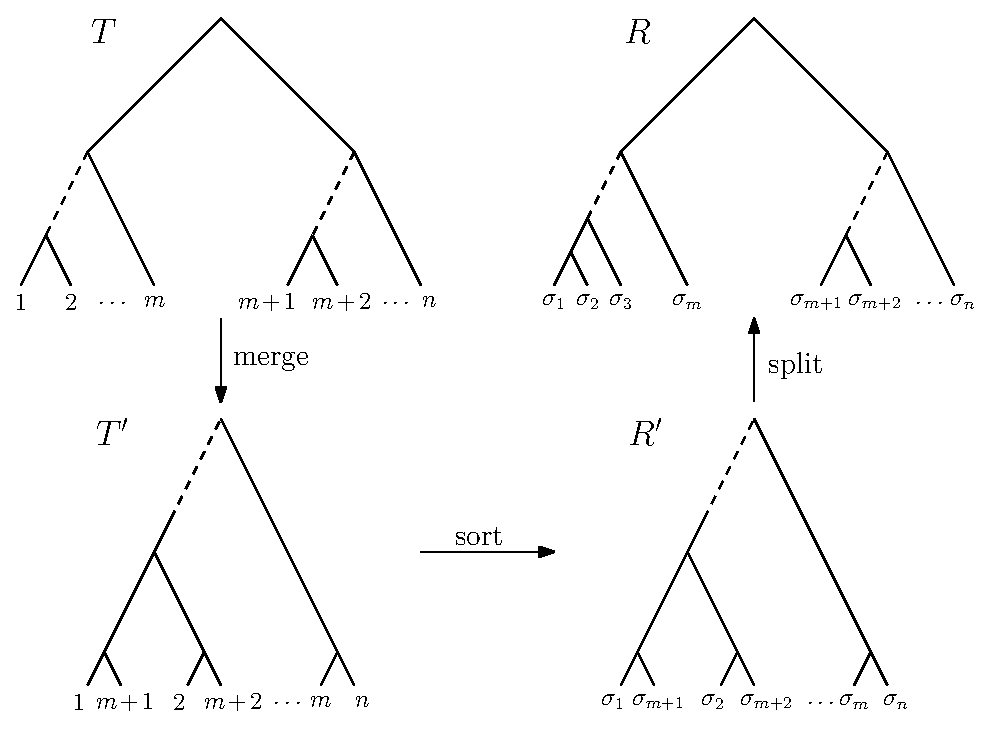
\includegraphics[width=.8\textwidth]{NNI_NP_proof}
\vspace{12pt}
\caption{Example of a shortest path between two trees $T$ and $R$ in $\nni$.
In \autocite{Li1996-zw} it is proven that there is a labelling that ensures that there is no shortest path in $\nni$ where the clusters (dots vs.\ squares) shared between $T$ and $R$ are preserved.
Instead, the depicted path where $\frac{n}{2}$ cherries are built and then sorted before being resolved is a shortest path}
\label{fig:NNI_NP_proof}
\end{figure}

Since the example of a shortest $\nni$ described above, which was used to prove Theorem~\ref{thm:split_nni} in \autocite{Li1996-zw}, does not work in $\rnni$, a contrary statement was conjectured in \autocite{Gavryushkin2018-ol}.
For understanding this conjecture it is important to know the connection between edges in a tree and so-called \emph{splits}, which are bipartitions of the taxon set of a tree:
By deleting an edge $e$ of a tree $T$ one receives two graphs with labels in $A$ and $B$, respectively, such that $\{A,B\}$ is a partition of the taxon set of $T$.
Note that each edge induces such a bipartition, often written as $A|B$, and that both edges incident to the root of a tree induce the same partition.
Since these partitions are commonly referred to as splits, the following conjecture was named \emph{Split Theorem} in \autocite{Gavryushkin2018-ol}.

\begin{conjecture}[Split Theorem]
For the $\rnni$ graph the following statement holds:
If a partition of leaves given by an edge is present in two trees $T$ and $R$ then the partition is presented in every tree on every shortest path between $T$ and $R$.
\label{conjecture:split_theorem}
\end{conjecture}

We found a simple counterexample to this conjecture, provided in Figure~\ref{fig:splitthm_counterexample}.

\begin{figure}[H]
\centering
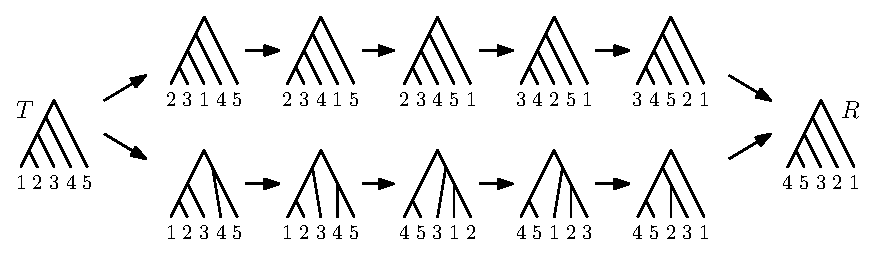
\includegraphics[width=\textwidth]{splitthm_counterexample}
\vspace{12pt}
\caption{The split $123|45$ is present in $T$ and $R$, but the path at the top is a shortest path (computed by $\csort$) where none of the trees contains this split.
On the path at the bottom, which is a shortest path as well, this split is maintained.}
\label{fig:splitthm_counterexample}
\end{figure}

Since the counterexample in Figure~\ref{fig:splitthm_counterexample} shows that the version of the Split Theorem stated in \autocite{Gavryushkin2018-ol} does not hold, we will now claim an alternative to this conjecture, the \emph{Cluster Theorem} (Conjecture~\ref{conjecture:cluster_theorem}).
The Cluster Theorem concerns clusters instead of splits.
This is motivated by the fact that rooted phylogenetic trees can uniquely be represented by sets of clusters \autocite{Steel2016-ye}, but not by sets of splits as they cannot define the position of the root.
Note that trees $T$ and $R$ in Figure~\ref{fig:splitthm_counterexample} induce the same set of splits, but share no cluster.

\begin{conjecture}[Cluster Theorem]
For the $\rnni$ graph the following statement holds:
if two trees $T$ and $R$ contain the same cluster $C$, then $C$ is present as cluster in every tree on every shortest path between $T$ and $R$.
\label{conjecture:cluster_theorem}
\end{conjecture}

For providing further evidence that the Cluster Theorem holds in $\rnni$, we could show computationally that it holds for the $\rnni$ graph on small trees with up to six taxa.
We did this by computing subgraph of $\rnni$ only containing trees that share a cluster and compare distances within this subgraph with distances in the whole $\rnni$ graph \autocite{Collienne2019}.
We computed these graphs according to the algorithm of \autocite{Gavryushkin2018-ol} as discussed in Section~\ref{section:algorithms}.

% \todo{LC: We still need to check 7 taxa.}
% We are doing this in the following way.
% We focus on the subset of trees that induce share a cluster.
% It is sufficient to consider clusters of the shape $\{1, \ldots, m\}$ for $2 \leq m \leq n-1$, because of the symmetry of the space:.
% distances $d(T_1,R_1)$ and $d(T_2,R_2)$ between two pairs of trees $(T_1,R_1)$ and $(T_2,R_2)$ are equal if one can receive $T_2$ from $T_1$ by permuting the taxa the same way as it is necessary for receiving $R_2$ from $R_1$.
% Therefore, we compute for all $m = 2, \ldots, n-1$ exact $\rnni$ distances between all pairs of trees containing the cluster $\{1, \ldots, m\}$, using Dijkstra's algorithm \autocite{Dijkstra1959-ph} on the $\rnni$ graph, which we can compute as explained in Section~\ref{section:alg_RNNI_graph}.
% Additionally, we compute the subgraph of $\rnni$ induced by the subset of trees that include the cluster $\{1, \ldots, m\}$.
% With the Floyd-Warshall algorithm we compute all pairwise distances between the trees in this subgraph and compare them with the distances in $\rnni$.
% With this approach it is possible to show that the Cluster Theorem holds for up to seven taxa.
% \todo{LC: We still need to check 7 taxa.}


% \section{Ideas}
%
% [This section includes some ideas that we could possibly include in the paper]
%
% Using the same argument as in the proof of Lemma~\ref{lemma:distance_delete_taxon} we can establish Proposition~\ref{proposition:lower_bound_distance} that provides a lower bound on the distance between trees.
%
% \begin{proposition}
% If trees $T$ and $R$ and taxon $x$ are such that $|\rank_T(\parent_T(x)) - \rank_R(\parent_R(x))| = \delta$ then $d(T,R) \geq \delta$.
% \label{proposition:lower_bound_distance}
% \end{proposition}
%
%
% The paths computed by $\findpath$ depend on the order of input trees $T$ and $R$:
% $\findpath(T,R)$ does not necessarily produce the reverse path of $\findpath(R,T)$.
% An example can be found in Figure~\ref{fig:findpath_not_symmetric}.
% However, simulations suggest that the lengths of the two paths computed by $\findpath$ for one pair of trees are equal.
%
% \begin{conjecture}
% Let $T$ and $R$ be ranked trees.
% The lengths of paths $\findpath(T,R)$ and $\findpath(R,T)$ are equal.
% \end{conjecture}
%
% \begin{figure}[H]
% \centering
% 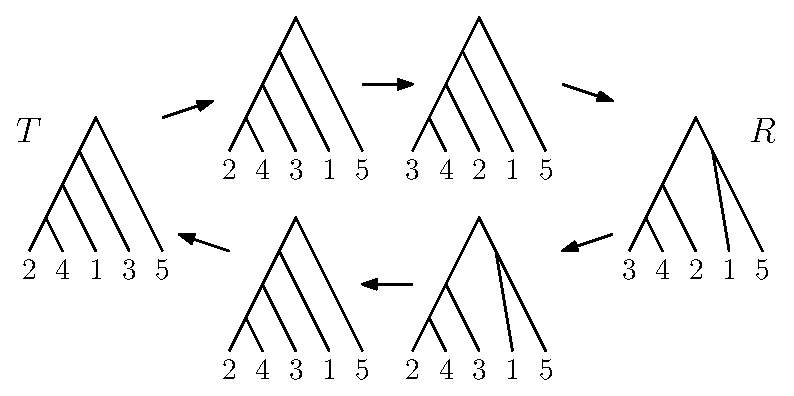
\includegraphics[width=0.7\textwidth]{findpath_not_symmetric}
% \vspace{12pt}
% \caption{Two paths computed by $\findpath$.
% At the top $\findpath(T,R)$, at the bottom $\findpath(R,T)$}
% \label{fig:findpath_not_symmetric}
% \end{figure}
%
% % idea for description of max distance caterpillar trees:
% \begin{lemma}
% Let $T$ and $R$ be caterpillar trees.
% It is $d_c(T,R) = \Delta(\rnni)$ if, and only if, $T$ and $R$ share no induced triplet.
% \todo{define induced triplets}
% \end{lemma}
%
% This Lemma does only hold for caterpillar trees and not for trees with more than one cherry.
% Furthermore, triplets do not represent ranked trees uniquely as they do not contain information about the ranks of internal nodes (but they can uniquely define caterpillar trees as these only have one cherry)
%
% \begin{proof}
% %TODO
% % Insert the proof here
% Fix $T = (\ldots(1,2) \ldots ,n)$, use induction on $n$ and $\csort$ (taxon $n$ must be in cherry of $R$ if distance is max).
% \end{proof}
%
% According to Algorithm~\ref{alg:max_dist_tree}, the number of trees with maximum distance to a given caterpillar tree $T$ is $(n-1)!$.
% The number of caterpillar trees with distance $\Delta(\rnni)$ from a given caterpillar tree is $2^{n-2}$.
%
%
% \subsection{Partition lattice}
%
% % Define Partition Lattice $\Pi_n$ and max chains in that lattice!
%
% \begin{theorem}
% The $\rnni$ graph on $n$ taxa is isomorphic to the graph of maximal chains of the partition lattice $\Pi_n$ where two maximal chains are connected by an edge if and only if they differ by exactly one partition.
% The corresponding metric spaces are isometric.
% \end{theorem}

\section{Discussion}

The aim of this paper was to gain better understanding of the $\rnni$ space of ranked phylogenetic trees.
Before investigating geometrical properties of $\rnni$ we introduced some algorithms in Section~\ref{section:algorithms}).
One of the most important algorithms we introduced here is $\findpath$, which can be used for approximating $\rnni$ distances.
We could in particular show that this algorithm computes exact distances for all pairs of trees on up to six taxa.
This algorithm might be a useful tool for future investigations of the $\rnni$ space.

We used the algorithms introduced in Section~\ref{section:algorithms} to prove some geometric properties of the $\rnni$ graph such as diameter and radius.
Moreover, we discovered that the set of caterpillar trees is convex in $\rnni$ (Theorem~\ref{thm:caterpillar_convex}).
With this result and the algorithm $\csort$ for computing shortest caterpillar paths (Section~\ref{section:alg_csort}) we can compute $\rnni$ distances between caterpillar trees in polynomial time.

This already suggests that there is a difference in complexity of computing distances in $\rnni$ and $\nni$, since in $\nni$ there is no subspace known for which computing distances only takes polynomial time.
In Section~\ref{section:cluster_theorem} we supported the claim that computing $\rnni$ distances is not as hard as computing $\nni$ distances further by discussing the proof of $\np$-completeness of computing distances in $\nni$ and showing that this proof does not work for $\rnni$.
Specifically, we conjectured the Cluster Theorem (Conjetcure~\ref{conjecture:cluster_theorem}), which does not hold in $\nni$.
However, we strongly suspect that it holds in $\rnni$ and could prove that it does hold for trees on up to six taxa \autocite{Collienne2019}.


\subsection{Open Problems}

In Section~\ref{section:cluster_theorem} we claimed that the Cluster Theorem holds for $\rnni$.
We could show that the previous version of it, the Split Theorem as it was conjectured in \autocite{Gavryushkin2018-ol}, is not true.
If the Cluster Theorem actually is true still remains an open question.
Proving it will be a big step towards finding the complexity of computing $\rnni$ distances.

This question of whether computing $\rnni$ distances is $\np$-hard is another problem for future research.
Though we did not aim to answer this question in this paper, we made some progress towards solving it by establishing some geometric properties of the $\rnni$ graph.
Comparing these results with what is known for the plain $\nni$ graph makes us assume that the complexity of computing shortest path in $\rnni$ might differ from $\nni$.
We also suspect that the fact that computing distances between caterpillar trees can be done in polynomial time might be the key for further investigation of the complexity of computing $\rnni$ distances.




\printbibliography

\end{document}
